\documentclass{beamer}
\usetheme{metropolis}           % Use metropolis theme

\usepackage{graphicx}
\graphicspath{ {../thesis/figures/} }
\usepackage{booktabs}
\usepackage{xspace}

\usepackage{amsmath}
\usepackage{amsfonts}
\usepackage{amssymb}
\usepackage{bm}
\usepackage{mathtools} % for \mathclap
\usepackage{nicefrac}
\usepackage[separate-uncertainty]{siunitx}
\usepackage{calc}
\newcommand\lasso{\textsc{lasso}\xspace}
\newcommand\fista{\textsc{fista}\xspace}
\newcommand\ista{\textsc{ista}\xspace}

\title{Integration of Prior Knowledge for Regression and
  Classification with Sparse Grids}
\date{November 15, 2016}
\author{Lukas Krenz}
\begin{document}
  \maketitle
  % \begin{frame}{Sparse Grids}
  %   \begin{figure}[H]
  %     \centering
  %   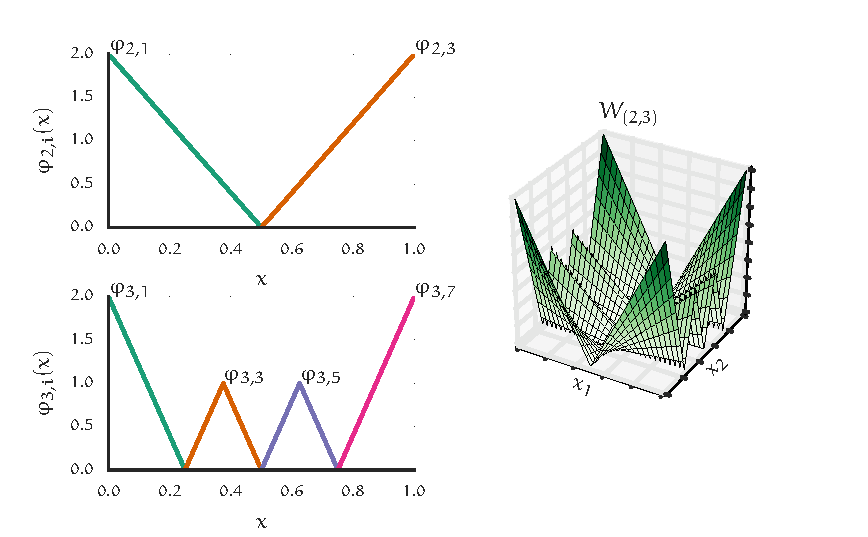
\includegraphics[width=\textwidth]{lin_mod_1d2d}
  %     \caption{Basis functions}
  %   \end{figure}
  % \end{frame}
  % \begin{frame}{Sparse Grids}
  %    \begin{columns}[T]
  %    \begin{column}[T]{0.5\textwidth}
  %      \begin{figure}[H]
  %        \centering
  %       \includegraphics[width=1\textwidth]{{{grid_T-inf}}}
  %        \caption{Full Grid}
  %      \end{figure}
  %    \end{column}
  %    \begin{column}[T]{0.5\textwidth}
  %      \begin{figure}[H]
  %        \centering
  %       \includegraphics[width=1\textwidth]{{{grid_T0}}}
  %        \caption{Sparse Grid}
  %      \end{figure}
  %    \end{column}
  %    \end{columns}
  % \end{frame}
  \begin{frame}{Feature Transformation}
     \begin{columns}[T]
     \begin{column}[T]{0.5\textwidth}
       \begin{figure}[H]
         \centering
        \includegraphics[width=1\textwidth]{{{circle}}}
         \caption{Original data}
       \end{figure}
     \end{column}
     \begin{column}[T]{0.4\textwidth}
       \begin{figure}[H]
         \centering
        \includegraphics[width=1.2\textwidth]{{{feature_trans}}}
         \caption{Transformed features}
       \end{figure}
     \end{column}
     \end{columns}
  \end{frame}
  \begin{frame}{Optimization Goal}
Model Matrix: \(p\) features \(\rightarrow\) \(m\) grid points
\begin{equation}
\bm{\Phi}(\bm{x}) = \begin{bmatrix}
\phi_1(x_1) & \phi_2(x_1) & \hdots & \phi_m(x_1) \\
\phi_1(x_2) & \phi_2(x_2) & \hdots & \phi_m(x_2) \\
\vdots & \vdots & \ddots & \vdots \\
\phi_1(x_n) & \phi_2(x_n) & \hdots & \phi_m(x_n)
\end{bmatrix}
\end{equation}

Optimization goal:
\begin{equation}\label{eq:optGoal}
\min_{\bm{\alpha}} \left\Vert  \bm{\Phi} \bm{\alpha} - \bm{y}   \right\Vert_2^2  + n \lambda \mathcal{S}(\bm{\alpha}) 
\end{equation}
  \end{frame}
  \begin{frame}{Tikhonov Regularization}
 Impose Gaussian Prior on the Weights
\begin{equation}\label{eq:diagonal-prior}
\bm{\alpha} \sim \mathcal{N} (0, \bm{\Gamma}^{-1})
\end{equation}

 \begin{equation}\label{eq:tik-langrangian}
  \mathcal{S}(\bm{\alpha}) = \Vert \bm{\Gamma} \bm{\alpha} \Vert_2^2
  \end{equation}

Improved Tikhonov matrix:
\begin{equation}\label{eq:diagonal-matrix}
\bm{\Gamma}_{i,i} = 4^{\vert \bm{l} \vert_1 - d}
\end{equation}
  \end{frame}
  \begin{frame}[plain]
    \begin{figure}[H]
      \centering
      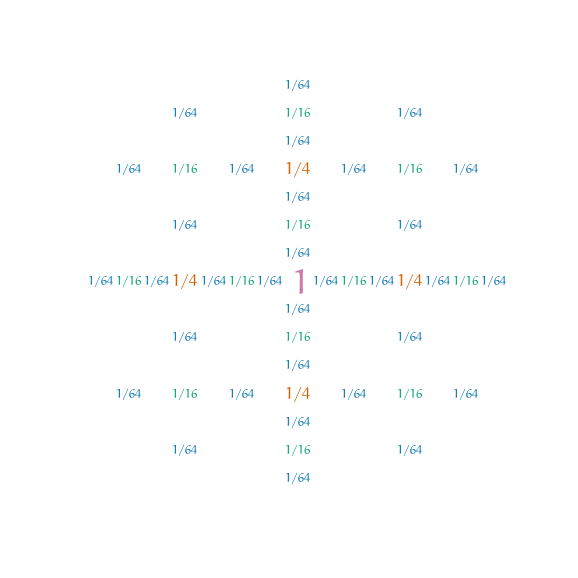
\includegraphics[width=1\textwidth, clip, trim={0 2.3cm 0 2cm}]{diagonal}
      \caption{The improved prior}
    \end{figure}
  \end{frame}
 

\begin{frame}{Tikhonov Regularization: Results Concrete}
\begin{figure}[H]
\centering
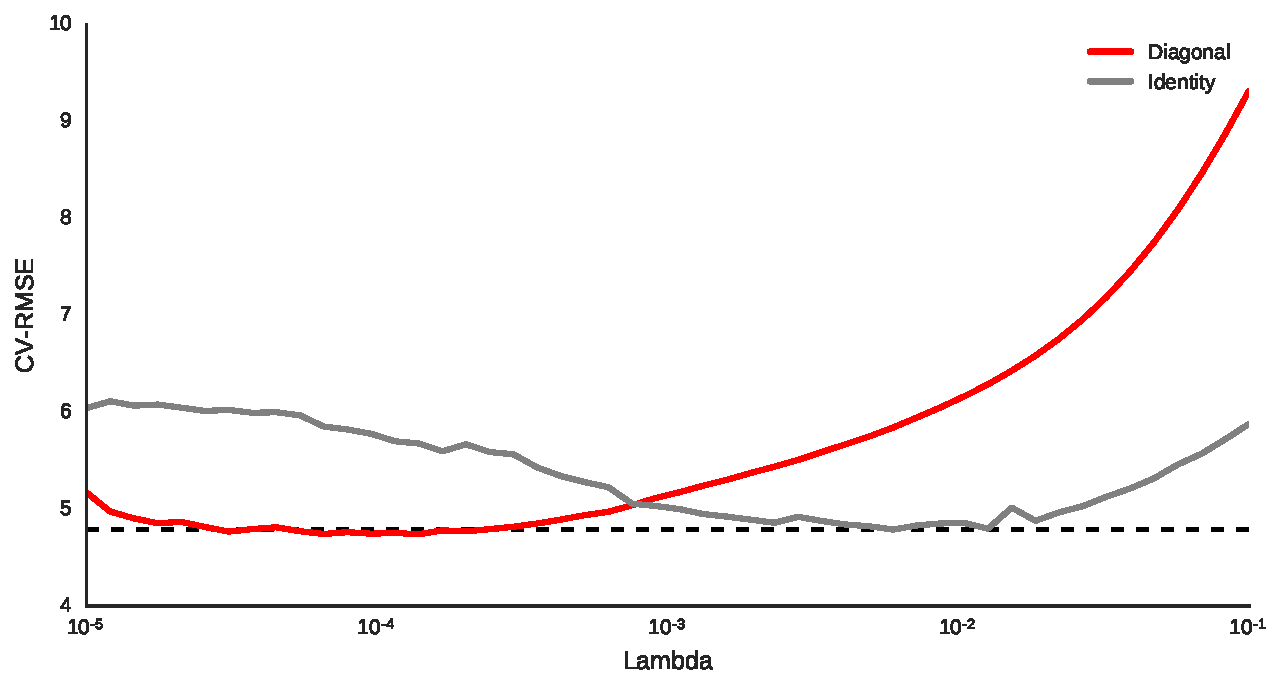
\includegraphics[width=\textwidth]{tikhonov_concrete_l5}
\caption{Results for the concrete dataset obtained with estimators with level
five for two different Tikhonov matrices}
\end{figure}
\end{frame}
   
\begin{frame}{Tikhonov Regularization: Results Power Plant}
\begin{figure}[H]
\centering
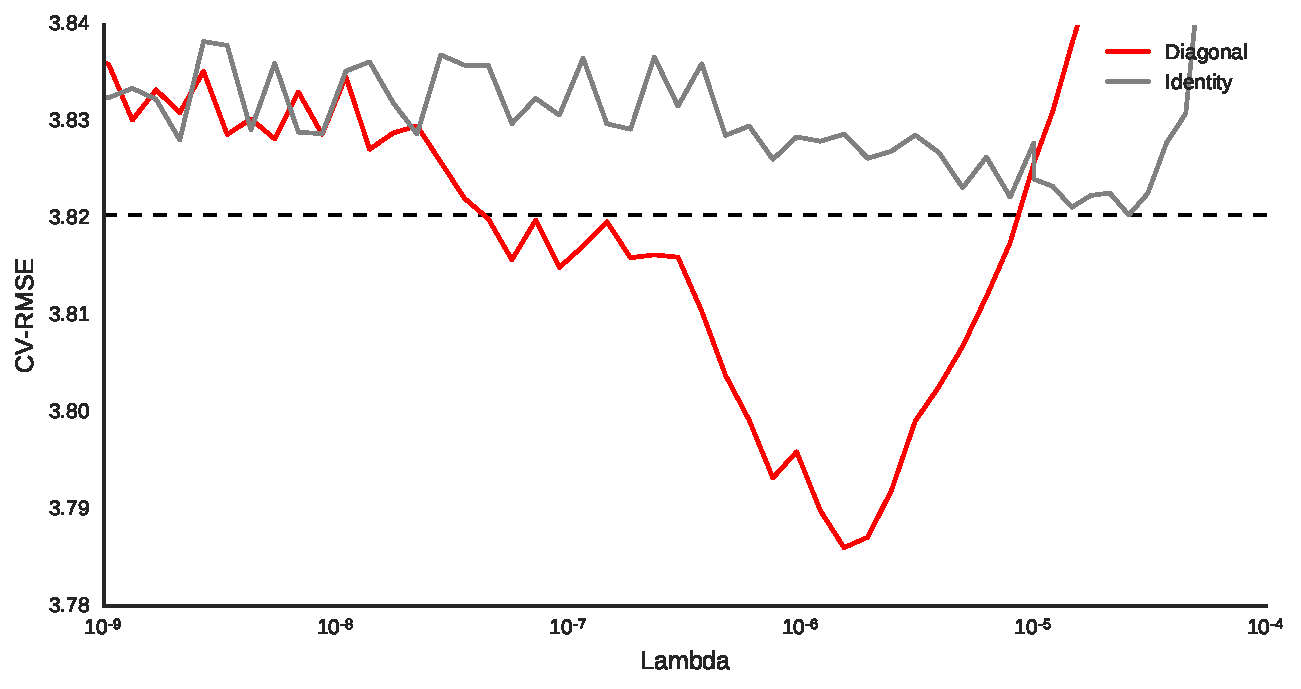
\includegraphics[width=\textwidth]{tikhonov_power_plant_l5}
\caption{Results for the power plant dataset obtained with estimators with level
five for two different Tikhonov matrices}
\end{figure}
   
  \end{frame}
  \begin{frame}{Sparsity-inducing Penalties: Lasso}
Sparsity-inducing penalty.

Sparsity: Weight vector \(\bm{\alpha}\), some entries are exactly zero.
 \begin{equation}
\mathcal{S}(\bm{\alpha}) = \Vert \bm{\alpha} \Vert_1
\end{equation}   
 \begin{figure}[tb]
    \centering
    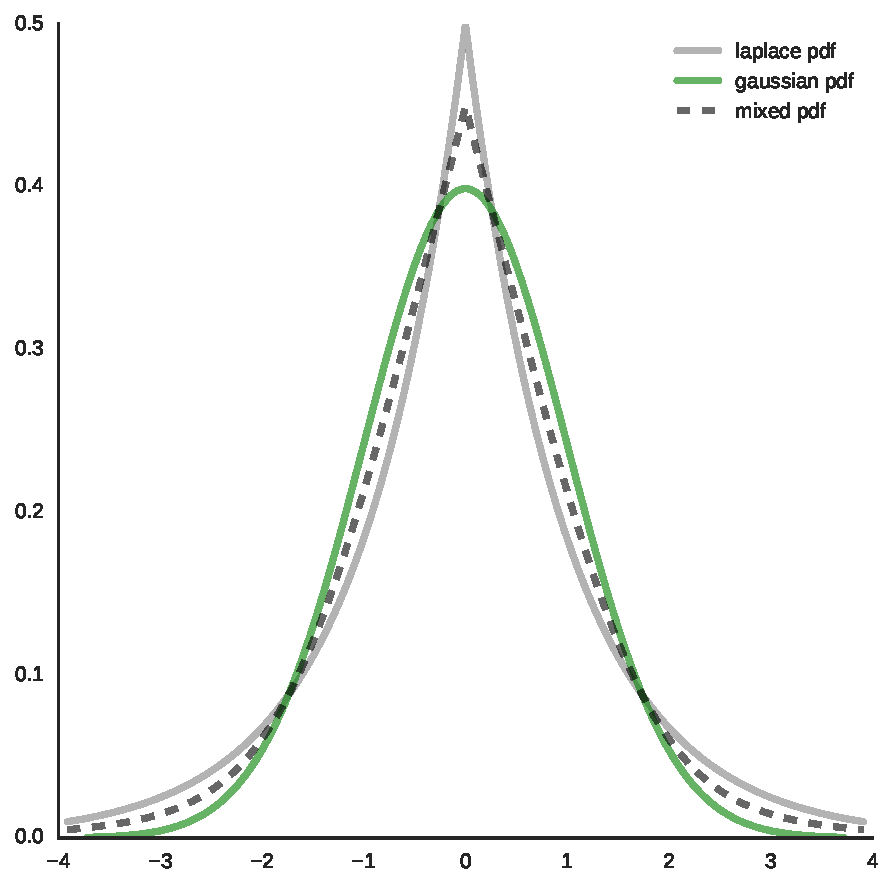
\includegraphics[width=0.7\textwidth]{pdfs}
    \caption{Plot of priors for ridge, lasso and elastic net}\label{fig:reg-pdfs}
\end{figure}  
  \end{frame}
  \begin{frame}{Sparsity-inducing Penalties: Elastic Net}
Combination of Tikhonov and lasso regularization:
\begin{equation}
  \mathcal{S}(\bm{\alpha}) = \left(1 - \theta \right) \Vert \bm{\alpha} \Vert_2  + \theta \Vert \bm{\alpha} \Vert _1
\end{equation}
Improved performance for highly-correlated features. 
  \end{frame}
  \begin{frame}{Sparsity-inducing Penalties: Group Lasso}
With \(\mathcal{P}\) as a partition of \(\bm{\alpha}\):
\begin{equation}
  \mathcal{S}({\bm{\alpha}}) = \sum_{\bm{p} \in \mathcal{P}} \left(\sqrt{\vert \bm{p} \vert}\right) \Vert  \bm{p} \Vert_2
\end{equation}
Group by order:
\begin{equation}
  \operatorname{order}(\bm{p}) = \vert \{ i\, \mid p_i \neq 0.5 \} \vert
\end{equation}
  \end{frame}
  \begin{frame}[plain]
\begin{figure}[hbt]
  \makebox[\textwidth][l]{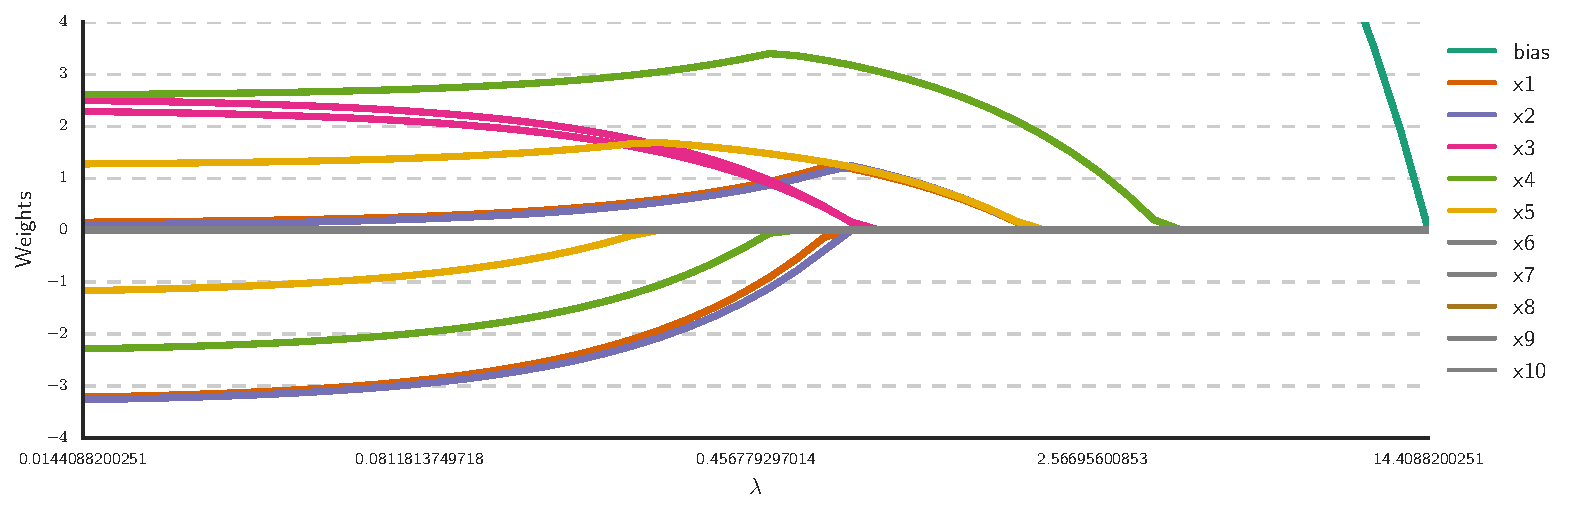
\includegraphics[width=1.1\textwidth]{path_lasso}}%
\end{figure}
\begin{figure}[hbt]
  \makebox[\textwidth][l]{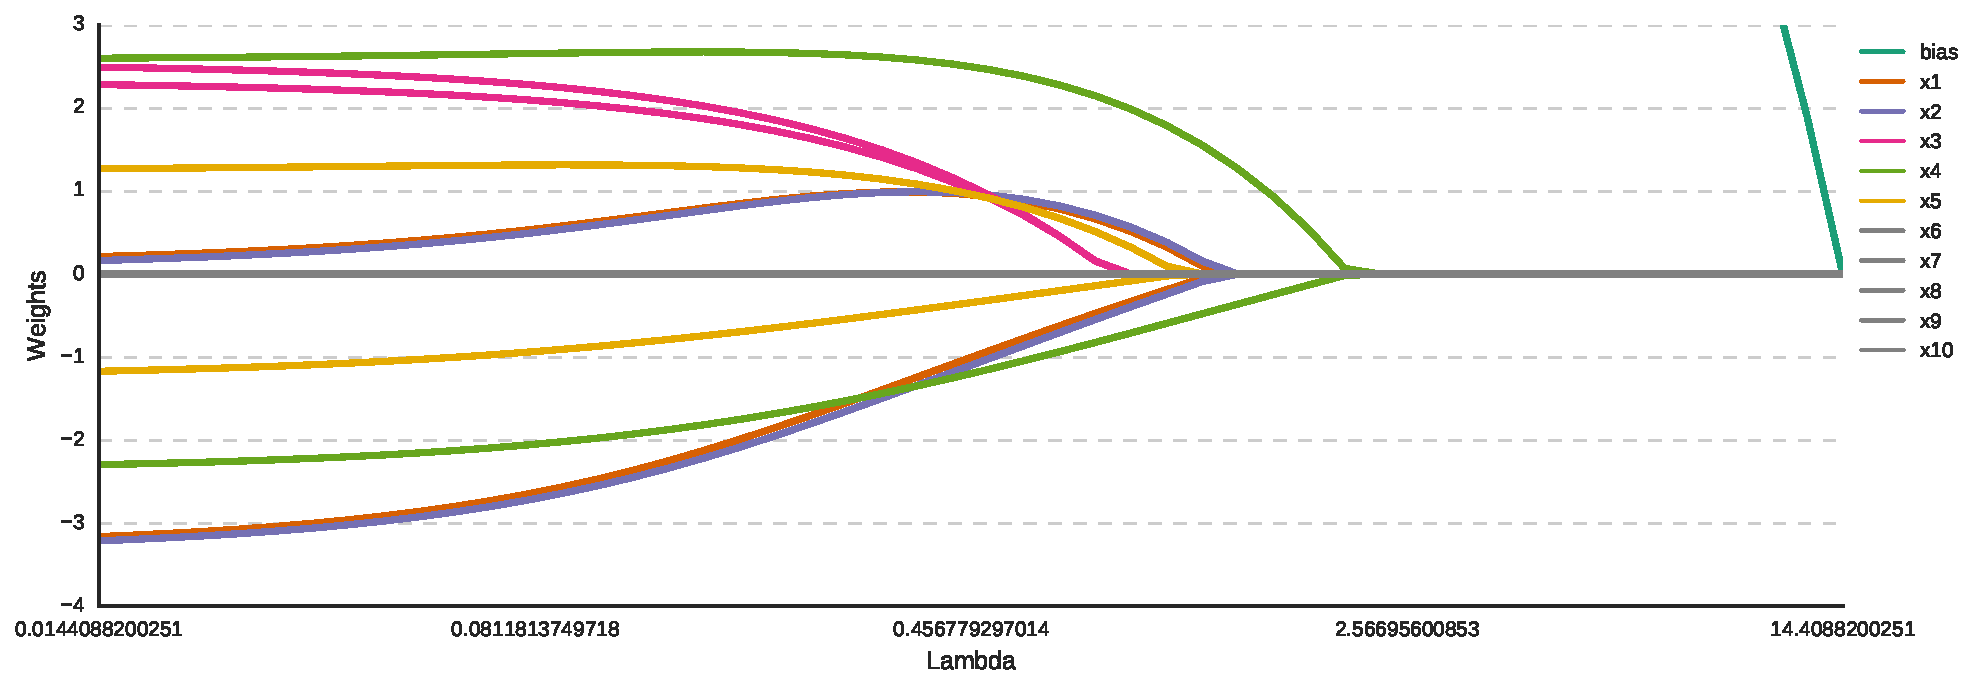
\includegraphics[width=1.1\textwidth]{path_grp}}%
\end{figure}

\end{frame}

\begin{frame}
  \frametitle{Sparsity-inducing Penalties: Results (1)}
\begin{table}[tb]
  \centering
   \begin{tabular}[c]{
    c
    S[table-format=1.4]
    }
  \toprule
\multicolumn{1}{c}{Reg.~Method}
& \multicolumn{1}{c}{\textsc{cv-rmse}}
     \\\midrule
Lasso & 4.582\\
Elastic Net ($\theta$ = 0.95) & 4.594\\
Group Lasso & 4.650\\
Ridge & 4.709 \\
\bottomrule
   \end{tabular} 
   \caption{Results for the concrete dataset for level five.}\label{fig:sparse-results}
\end{table}
\end{frame}

\begin{frame}
  \frametitle{Akaike Information criterion}
  Asymptotically equivalent with leave-one-out cross-validation.
  \begin{align}
  \operatorname{\text{Aic}}(\text{df}, \text{mse}) = 2\operatorname{df} + n \ln{(\text{mse})} + \text{constant}
\end{align}
Df.~are degrees of freedom.
For Lasso:
\begin{align*}
  \operatorname{df}(\bm{\Phi, \alpha}) &= \operatorname{rank}(\bm{\Phi}_{\bm{\mathcal{A}(\alpha)}}) \intertext{with}
  \bm{\mathcal{A}}(\bm{\alpha}) &= \{a \in \bm{\alpha}\,|\,a \neq 0\}
\end{align*}
For ridge:
\begin{equation*}
 \operatorname{df}(\bm{\Phi}, \lambda) = \sum_i \frac{\sigma_i^2 - \lambda}{\sigma_i^2}
\end{equation*}
\end{frame}

\begin{frame}{Sparsity-inducing Penalties: Results (2)}
    \centering
   \begin{tabular}[c]{S[table-format=1]
    c
    c
    S[table-format=3.1] %df
    S[table-format=4.2] %aic 
    S[table-format=2.3]}%rmse - test
  \toprule \multicolumn{1}{c}{Level}
& \multicolumn{1}{c}{Reg.~Method}
& \multicolumn{1}{c}{Gridsize}
& \multicolumn{1}{c}{\textsc{df}}
& \multicolumn{1}{c}{\textsc{Aic}}
& \multicolumn{1}{r}{Test-\textsc{rmse}}\\
     \midrule
5 & Ridge & 6650 & 716.7 & 2796.22 & 4.184 \\
4 & Lasso & 1382 & 518.0 & 2797.09 & 3.850 \\
4 & Ridge & 1470 & 558.0 & 2991.22 & 4.198 \\
5 & Lasso & 6632 & 754.0 & 2997.94 & 3.737 \\
\bottomrule
   \end{tabular} 
\end{frame}

\begin{frame}{Generalized Sparse Grids}
 New hyper-parameter \(T\), controls the granularity of the grid 

\begin{columns}
  \centering
  \begin{column}[b]{0.23\textwidth}
    \centering
    \includegraphics[width=\textwidth]{{{grid_T-inf}}}

    \(T = -\infty\)
  \end{column}
   \begin{column}[b]{0.23\textwidth}
    \centering
    \includegraphics[width=\textwidth]{{{grid_T0}}}

    \(T =0\)
  \end{column}
 \begin{column}[b]{0.23\textwidth}
    \centering
    \includegraphics[width=\textwidth]{{{grid_T0.5}}}

    \(T = 0.5 \)
  \end{column}
 \begin{column}[b]{0.23\textwidth}
    \centering
    \includegraphics[width=\textwidth]{{{grid_T1.0}}}

    \(T = 1\)
  \end{column}
\end{columns}
\end{frame}

\begin{frame}{Generalised Sparse Grids: Interaction terms}
    \includegraphics[width=\textwidth]{{{interactionT2}}}
\end{frame}

\begin{frame}
  \frametitle{Generalized Sparse Grids: Results}
  \begin{table}[h]
\centering
\begin{tabular}[c]{
  S[table-format=1.1]
  S[table-format=1]
  S[table-format=4]
  S[table-format=2.4]}
  \toprule \multicolumn{1}{c}{T}
& \multicolumn{1}{c}{Level}
& \multicolumn{1}{c}{Gridsize}
& \multicolumn{1}{c}{Root mean error}
\\\midrule
0 & 5 & 6650 & 4.184\\
0 & 4 & 1470 & 4.198\\
0.5 & 5 & 1180 & 3.797\\
\bottomrule
\end{tabular}
\caption{
  Errors of generalized grids for the concrete dataset.
}\label{fig:results-opt}
\end{table}
\end{frame}


\begin{frame}{Interaction-Term aware Sparse Grids}
  Idea: Only include some interaction terms. 
  \begin{columns}[b]
  \begin{column}{0.5\textwidth}
  \begin{figure}[H]
    \centering
    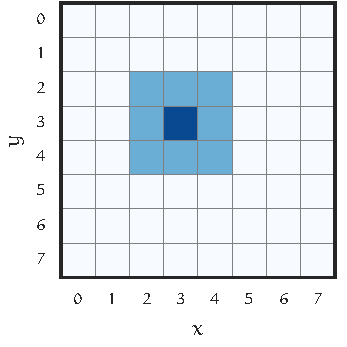
\includegraphics[width=0.9\textwidth]{nn_l2}
    \caption{\(3 \times 3\) Neighborhood}
  \end{figure}
  \end{column}
  \begin{column}{0.5\textwidth}
    \begin{figure}[H]
      \centering
      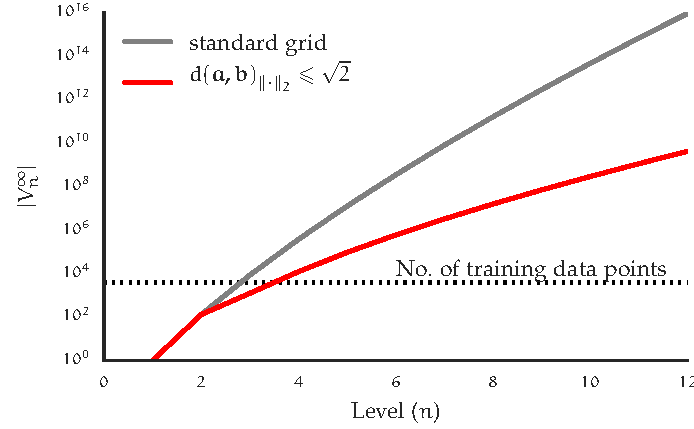
\includegraphics[width=1.0\textwidth]{interaction_sizes}
      \caption{Effect on grid size}
    \end{figure}
  \end{column}  \end{columns}
\end{frame}

\begin{frame}
  \frametitle{Optical Digits}
  \begin{figure}[H]
    \centering
    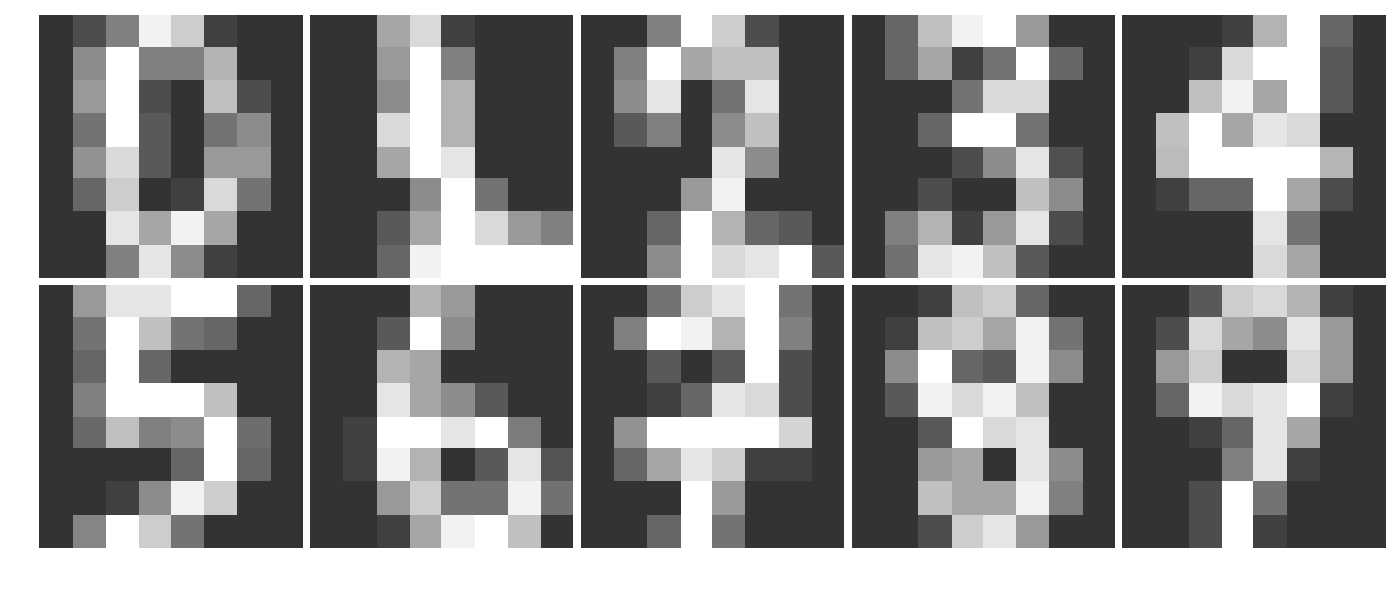
\includegraphics[width=\textwidth]{optdigits}
    \caption{Digits}
  \end{figure}
\end{frame}

\begin{frame}
  \frametitle{Optical Digits: Results}
 \begin{table}[h]
\centering
\begin{tabular}[c]{
  r
  S[table-format=1]
  r
  S[table-format=4]
  S[table-format=2.2]}
  \toprule \multicolumn{1}{r}{Sparse Grid Method}
& \multicolumn{1}{r}{Level}
& \multicolumn{1}{r}{Neighbors}
& \multicolumn{1}{r}{Gridsize}
& \multicolumn{1}{r}{Accuracy[\%]}
\\\midrule
Standard & 2 & all & 129 & 92.77\\
Interaction-Aware  & 3 &  \(3 \times 3\) & 1225 & 97.33\\
Adaptive & 2 & all & 1760 & 97.74\\
Interaction-Aware & 3 & \(5 \times 5\) & 2569 & 97.83\\
Standard & 3 & all & 8449 & 98.22\\
\bottomrule
\end{tabular}
\caption{
  Accuracy of sparse grids models for the optical digits dataset.
}\label{fig:results-opt}
\end{table} 
\end{frame}

\begin{frame}
  \frametitle{Conclusion}
  \begin{itemize}
  \item Competitive results
  \item Prior knowledge $\rightarrow$ better \& more effective solutions
  \item Only mild assumptions
  \end{itemize}
\end{frame}

\end{document}


%%% Local Variables: 
%%% coding: utf-8
%%% mode: latex
%%% TeX-engine: xetex
%%% TeX-master: t
%%% End: 